\subsection{Problem statement}
\label{subsec:problem-statement}

The Discovery~\footnote{\url{https://discovery.ic.unicamp.br/}} laboratory, located at \ac{UNICAMP}~\footnote{\url{https://ic.unicamp.br/}}, is working on a seismic analysis project with Petrobras~\footnote{\url{https://petrobras.com.br/}}.
This project aims at developing a framework called \ac{DASF}~\cite{dasf}, which facilitates the execution of machine learning algorithms and seismic attribute operators on computing clusters.
However, the inputs of the graphs created for seismic analysis are massive datasets that can contain terabytes of data.
Even supercomputers do not have enough memory to handle the computation on a single node.
Therefore, usually, the execution is distributed by using data parallelism.

To facilitate this process, \ac{DASF}~\cite{dasf} has a parameter called "block size."
With the value of that parameter, \ac{DASF}~\cite{dasf} uses Dask's~\cite{dask} automatic chunking feature to split the dataset into chunks.
However, setting this parameter can be challenging because it requires finding the optimal relationship between it and the network overhead caused by it.

To illustrate this challenge, image~\ref{fig:block-size} presents three computing graphs receiving input data from a seismic dataset.
The first scenario (on the left) illustrates the situation in which the input data is processed as a whole, which requires a significant amount of memory to store the data during the execution and fails due to lack of memory.
The second scenario (in the middle) divides the data into thousands of small parts, reducing the memory requirements but adding network and scheduler overhead.
The third scenario (on the right) divides the data into smaller parts, minimizing network and memory requirements.

\begin{figure}[ht]
  \caption{Block size impact on memory and network usage}
  \label{fig:block-size}
  \resizebox{\textwidth}{!}{%
    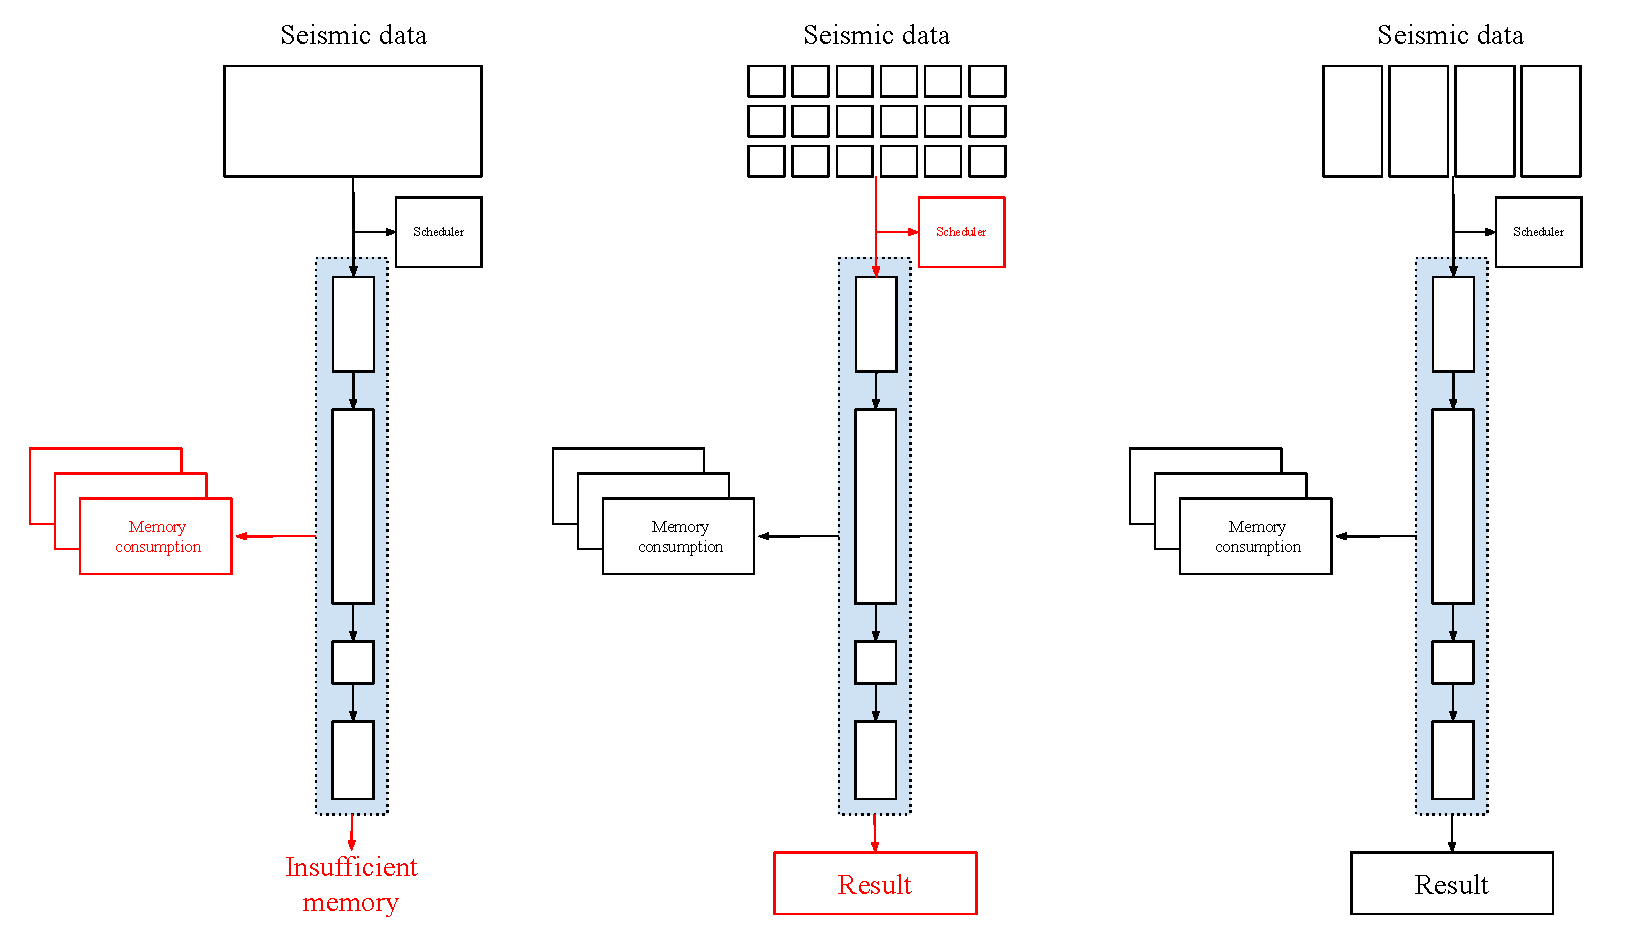
\includegraphics{block-size.pdf}
  }
\end{figure}

While executing the graph, the user must manually set the block size parameter.
Setting a large value may lead to memory issues and cause significant delays due to the trial-and-error nature of the execution flow.
Since Petrobras uses supercomputers to execute those graphs, this delay may be even more significant considering the time it takes to submit a job due to the queue waiting time.

On the other hand, setting a small block size value may increase the execution time due to network and scheduler overhead.
Since Petrobras has many graphs to execute, and the complete execution of each usually takes a long time, optimizing the block size parameter may lead to considerable efficiency improvements by reducing the number of failed jobs on their clusters and removing the need to tune that parameter manually.

Dask~\cite{dask} provides an automatic chunking feature, but it relies on the chunk size parameter, which is a static parameter defined before execution.
Figuring out that parameter for algorithms that do not require a large working memory is easy since the developer can set that to a percentage of the available memory.
However, some seismic operators used by Petrobras generate a large working memory during the graph execution, which makes it difficult to determine the ideal chunk size.

Based on this assumption, if someone predicts the memory usage of the graph, that person can use Dask's~\cite{dask} auto chunking feature to split the data into the ideal number of chunks automatically.
Since \ac{DASF}~\cite{dasf} uses Dask~\cite{dask} under the hood, the block size parameter on \ac{DASF}~\cite{dasf} is equivalent to the chunk size parameter on Dask~\cite{dask}.
Therefore, this research aims to develop a way to understand the memory footprint of a graph to simplify and automate the decision of the ideal chunk size.

As a practical usage, this research aims to create a \ac{DASF}~\cite{dasf} plugin that can automatically set the optimal block size parameter during execution based on a machine learning model that can predict the memory usage requirements of the graph.
That plugin will help \ac{DASF}~\cite{dasf} users to optimize resource utilization and minimize waiting and execution time.
The model will provide a comprehensive understanding of memory usage patterns for different block sizes and contribute to developing a more efficient data partitioning strategy to execute a graph in large-scale clusters.
